\section{Word to word models} \label{sec: w2w models}
The more difficult challenge lies in unannotated texts without a paradigm for pairing words of an example data set. In this manner a language normally occurs and is learned by humans. A priori one has to expect results of poorer quality in comparison to the configuration of \secreff{subsec: first model and architecture} because they were tailored and \gls{nlp} comes always with uncertainties.

% - - - - - - - - - - - - - - - - - - -

\subsection{Data preparation} \label{sec: data preparation}
The data is extracted from two books, namely ``Gut gegen Nordwind'', written by Daniel Glattauer in German~\cite{Glattauer06GGW} and from Jostein Gaarder ``Sophie's World''~\cite{Gaarder96SW} in English. Two languages were chosen since German comes in general with a high degree of freedom in word order, in comparison English is more restrictive. This distinction may be important, since analyzing successive words is fundamental for this work. Because the books are available as \texttt{pdf}-file, the python module \pymupdf{}~\cite{pymupdf} is used to generate a simple \texttt{String} containing the whole text, which is afterwards parsed by \spacy{}~\cite{spacy2}. This is a powerful tool in the area of \gls{nlp} and some techniques are indispensable for further analysis, mainly
\begin{itemize}
	\item Tokenization: segmenting text into words, punctuations marks etc.
	\item \gls{pos}-Tagging\footnote{More information on \cite{udpostags}}: assigning word types to tokens, like verb or noun \label{item: pos tag}
	\item Lemmatization: assigning the base forms of words\footnote{For example, the lemma of “was” is “be”, and the lemma of “rats” is “rat”.}
	\item word2vec~\cite{MikolovEtAl13DRW, MikolovEtAl13EEW}: calculating a vector representation with real values of a word, in the following called \emph{word vector}.
\end{itemize}
%Lemmatization and Part-of-speech (POS) Tagging are used for bookkeeping and result evaluation.
%
Additionally, a mechanism was implemented to extract an exact number of words having equal sized foundations in both languages. The training data consists of word pairs in their occurring order, for instance the sentence
\begin{quote}
	Goethe remarked about Alexander von Humboldt to friends that he had never met anyone so versatile.\footnote{Sentence taken from \cite{Wulf16ION}} %\footcite{Wulf16ION}
\end{quote}
gets tokenized, lemmatized and coupled having
\begin{verbatim}
	("Goethe", "remark"), ("remark", "about"), ("about", "Alexander"), ...
\end{verbatim}
where the first component serves as input and the second one as supervised output.

Clearly, not the actual word is fed into the Neural Network, but numerical representations: either a \onehot{} or a word vector. To construct the former, the concept of the \cognitiveroom{} is applied by building a list containing all words of the text \ie one word resembles one state and states are encoded by place cells. To learn the transition probability matrix, as proclaimed at the beginning of the chapter, one has to transform the prediction of the Neural Network into a probability vector via division by its sum. This processing is done not during training because it is supervised via \onehot{s}.

% --------------------------------------

\subsection{\onehot{} approach} \label{subsubsec: onehot approach}
This configuration follows the principles of the first model (\secreff{subsec: first model and architecture}) by using \onehot{s} as input and output but there are no invented grammatical rules anymore. The training data is now directly related to concrete words and not to a word class. An illustration of the data structure is given in \figref{\ref{fig: text model graph ohe w2v}}.

% --------------------------------------

\subsection{Word vector approach} \label{subsubsec: word vector approach}
The Neural Network takes word vectors, a $ 300d $-vector of real numbers, as input and omits them during training. Word vectors are calculated by \spacy{}. To be precise, this step has two stages. Building the training data is easy because it is effortlessly possible to retrieve the real valued vector given a word. Since predictions aren't (and can't be) as accurate as the results \spacy{} computes, it is impossible to query a dictionary or database to reshape the exact word. For such situations, the module offers the option to retrieve a list with the $ n \in \mathbb{N} $ closest words. This list includes the $ n $ words whose vector representations have the smallest euclidean distance to the desired vector \ie the prediction.

In the next step, a check is performed whether the word is part of the book \ie the \cognitiveroom{}. If so, the euclidean distance is taken as entry in the Transition Probability Matrix $ T $, which will undergo a row-wise transformation to fit the criteria of a transition probability matrix. One disadvantage is an ambiguous prediction and therefore a less sharp $ T $. But in comparison to the \onehot{}, a word vector bears a lot more information, which hopefully can be exploited by the neural network. The data structure is shown in \figref{\ref{fig: text model graph ohe w2v}} next to the \onehot{} equivalent.

\begin{figure}
    \centering
        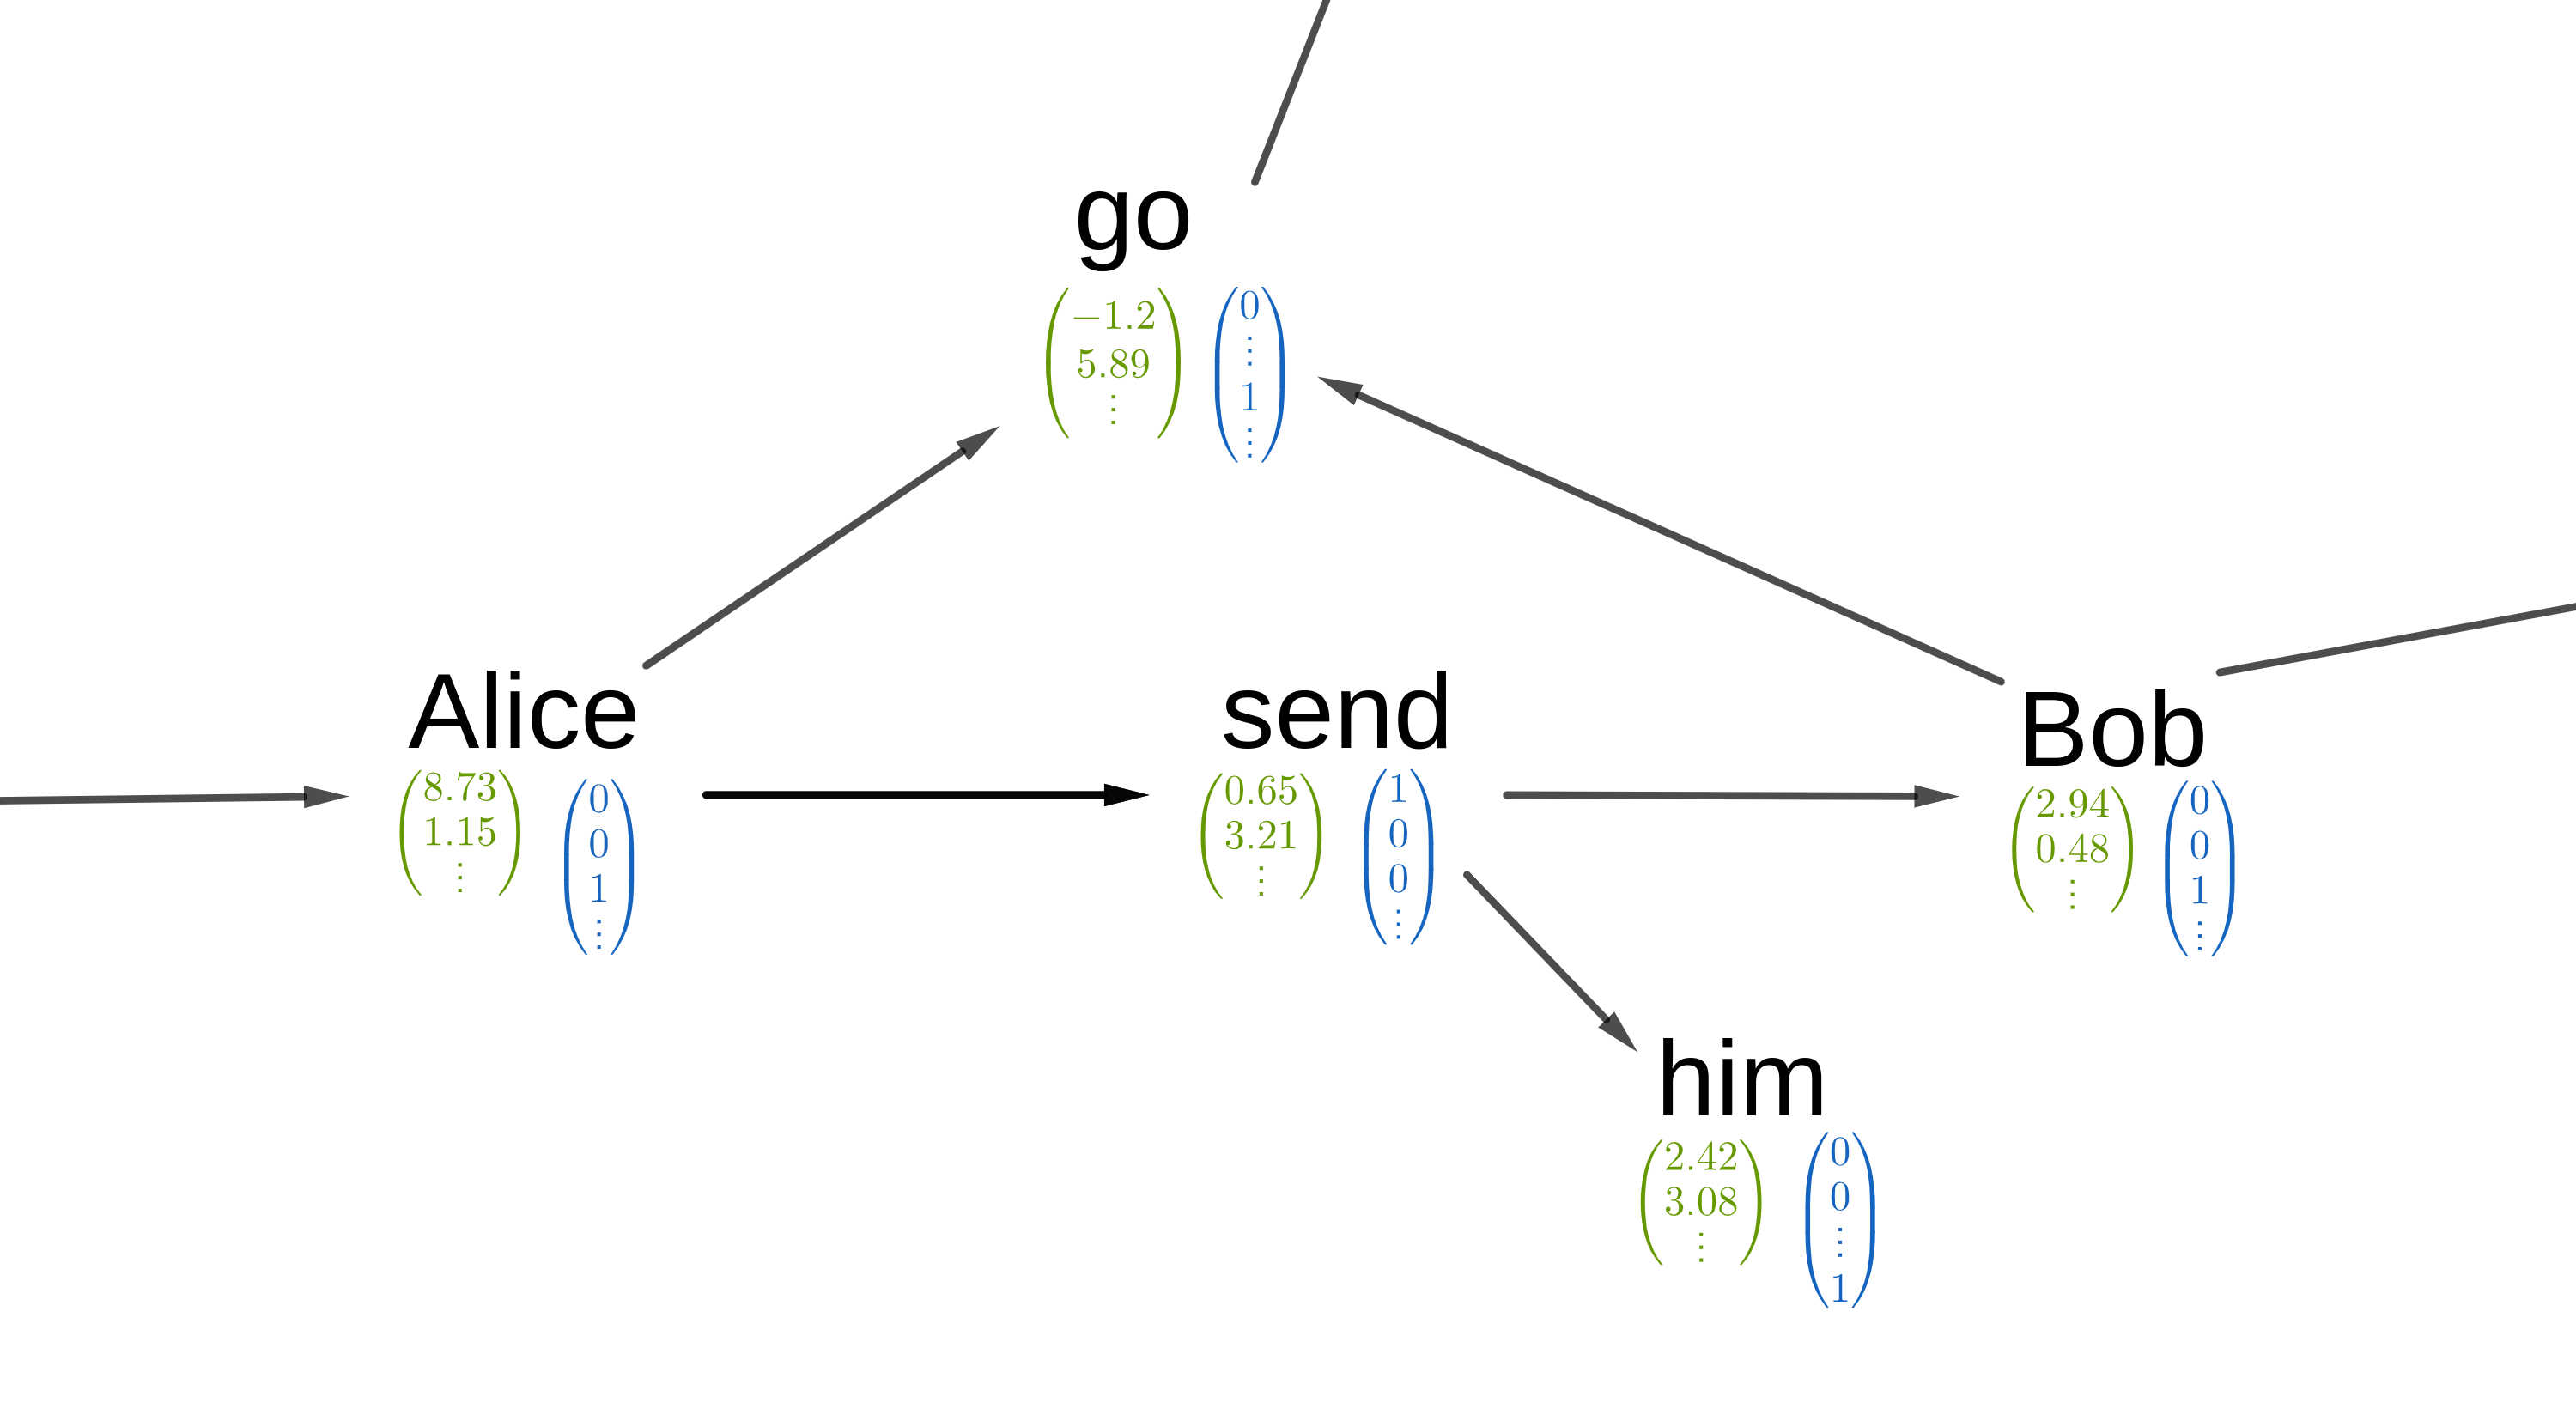
\includegraphics[width=\linewidth]{Bilder/Graphen/w2w_ohe_w2v.png}
    \caption{The word to word models can also be illustrated as graphs, though more complex. The lemmatized words of the text serve as vertices and the pairs mentioned before in \secreff{sec: data preparation} as edges. In green are word vectors and in blue \onehot{s} denoted. This cropped graph is generated by the bold passages of the text: ``\textbf{Alice sends Bob} a message. \textbf{Alice goes} to the grocery store. Peter \textbf{sent him} a letter. \textbf{Bob went} to his friend.''}
    \label{fig: text model graph ohe w2v}
\end{figure}

% --------------------------------------

%\subsection{Combined approach} \label{subsubsec: combined approach}
%The third model blends in both approaches by using the word vectors as input and a \onehot{} as output. It's goal is to tackle the imprecision aspects of the inevitable blur the word vector configuration experiences.
